
\documentclass[12pt,a4paper]{article}
\usepackage[margin=2cm]{geometry}
\usepackage{indentfirst}
\usepackage[utf8]{inputenc}
\usepackage[T1]{fontenc}
\usepackage{longtable}
\usepackage{booktabs}
\usepackage{array}
\usepackage{graphicx}
\usepackage{titling}
\usepackage{float}
\usepackage{hyperref}
\usepackage{tikz}
\usepackage{amsmath}
\usetikzlibrary{shapes, arrows, positioning, shadows}
\usepackage[justification=centering]{caption}
\usepackage{subcaption} 
\usetikzlibrary{shapes.geometric, arrows.meta, positioning}
\geometry{left=1.5cm, right=1.5cm, top=2cm, bottom=2cm}
 
\renewcommand{\maketitle}{%
  \begin{titlepage}
    \centering
    
    \vspace*{0.5cm}
 
    {\LARGE \textbf{EVALUASI TENGAH SEMESTER} \par}
    {\LARGE \textbf{MATA KULIAH PEMROGRAMAN KONTROLLER} \par}
 
    \vspace{1cm}
 
    {\large \textbf{Dosen Pengampu: Ahmad Radhy, S.Si., M.Si} \par}
 
    \vspace{1.5cm}
 
    
\includegraphics[width=8cm]{its_logo.png} 
 
    \vspace{2cm}
 
    {\large Disusun oleh (Kelompok 3): \par}
    \vspace{0.5cm}
    {\large \textbf{Ahmadin Fatkhurahman} \normalsize (NRP: 2042241015) \par}
    \vspace{0.2cm}
    {\large \textbf{Ghani Raihan Syakir} \normalsize (NRP: 2042241036) \par}
    \vspace{0.2cm}
    {\large Kelas: \textbf{4C} \par}

    \vfill
 
    {\normalsize
      \textbf{PRODI D4 TEKNOLOGI REKAYASA INSTRUMENTASI} \\
      \textbf{DEPARTEMEN TEKNIK INSTRUMENTASI} \\
      \textbf{FAKULTAS VOKASI} \\
      \textbf{INSTITUT TEKNOLOGI SEPULUH NOPEMBER} \\
      \textbf{2025} \par
    }
 
  \end{titlepage}%
}
 
\title{}
\author{}
\date{}
 
\begin{document}
\maketitle

\section*{A. Studi Literatur}

Bagian ini menyajikan analisis komprehensif terhadap 15 artikel jurnal ilmiah internasional bereputasi (IEEE Xplore/Scopus) dalam rentang publikasi 2021-2026. Kajian pustaka ini difokuskan secara terarah pada penelusuran teknologi sistem kendali terintegrasi antara \textit{Basic Process Control System} (BPCS) dan \textit{Safety Instrumented System} (SIS), manajemen redundansi sensor untuk meningkatkan \textit{availability}, implementasi bahasa pemrograman Rust untuk menjamin \textit{high-integrity} pada sistem tertanam kritikal, serta optimasi performa pada arsitektur mikrokontroler modern berbasis ESP32-S3. Ringkasan dari tata metodologi, hasil utama, beserta arah \textit{future work} yang disarankan oleh masing-masing peneliti disajikan secara terstruktur pada Tabel 1 di bawah ini.

\begin{small}
\begin{longtable}{|c|>{\raggedright\arraybackslash}p{3cm}|>{\raggedright\arraybackslash}p{4cm}|>{\raggedright\arraybackslash}p{4cm}|>{\raggedright\arraybackslash}p{4cm}|}
\caption{Ringkasan 15 Jurnal Acuan (2021--2026)} \label{tab:literatur} \\
\hline
\textbf{No} & \textbf{Judul \& Penulis Lengkap (Tahun)} & \textbf{Metode} & \textbf{Hasil Utama} & \textbf{Future Work} \\
\hline
\endfirsthead
\caption[]{Ringkasan 15 Jurnal Acuan (2021--2026) - Lanjutan} \\
\hline
\textbf{No} & \textbf{Judul \& Penulis Lengkap (Tahun)} & \textbf{Metode} & \textbf{Hasil Utama} & \textbf{Future Work} \\
\hline
\endhead
\hline
\endfoot

1 & Analyzing and Comparing DL Models on ARM 32-bit MCU (Aurélien Benoit, Christophe Escriba, David Gauchard, Alain Esteve, \& Carole Rossi, 2024) & Penelitian ini menerapkan evaluasi komparatif terhadap sembilan variasi arsitektur Deep Learning (seperti CNN, LSTM, dan GRU) yang dikompresi menggunakan TensorFlow Lite for Microcontrollers. Data triaksial akselerometer diproses melalui jendela geser (\textit{sliding window}) pada mikrokontroler ARM Cortex-M4 untuk mendeteksi anomali jatuh secara \textit{on-device}. & Model CNN DENSE menunjukkan performa paling optimal dengan akurasi 94,70\% dan konsumsi arus sangat rendah sebesar 6,72 mA. Hasil ini membuktikan bahwa algoritma Deep Learning yang kompleks dapat berjalan pada unit daya baterai terbatas dengan tetap memberikan \textit{lead time} deteksi jatuh yang aman bagi pengguna medis (176,91 ms). & Pengembangan selanjutnya disarankan untuk mengimplementasikan \textit{Spiking Neural Networks} (SNN) guna menekan konsumsi daya hingga tingkat mikro-watt. Selain itu, diperlukan validasi pada subjek lansia secara langsung di lingkungan luar ruangan (\textit{outdoor}) untuk memperkuat generalisasi model terhadap gangguan data sensor visi. \\ \hline

2 & Task-Specific Energy Profiling for MCU Selection (Uttunga G. Shinde, Timm Luhmann, Johannes Klueppel, Till Steinmann, Laura M. Comella, Wanli Yu, Stefan J. Rupitsch, \& Peter Woias, 2025) & Metodologi penelitian menggunakan instrumen Joulescope untuk melakukan pengukuran konsumsi daya \textit{real-time} berbasis siklus instruksi CPU. Profiling energi dilakukan pada tingkat tugas (\textit{task-specific}) meliputi proses akuisisi sensor, komputasi data, dan transmisi nirkabel LoRa pada mikrokontroler Ambiq Apollo 3 dan Texas Instruments MSP430. & Mikrokontroler Ambiq Apollo 3 ditemukan memiliki efisiensi energi 19,84\% lebih tinggi dibandingkan arsitektur pesaing dalam kondisi beban kerja aktif. Integrasi \textit{Real-Time Clock} (RTC) eksternal dan manajemen register tingkat rendah terbukti mampu menurunkan konsumsi daya mode tidur hingga 62\% pada aplikasi otonom jangka panjang. & Fokus penelitian di masa depan diarahkan pada pembuatan model manajemen daya adaptif yang mengintegrasikan unit \textit{energy harvesting}. Peneliti juga menekankan pentingnya melakukan uji banding serupa pada arsitektur RISC-V terbuka untuk mengevaluasi efisiensi daya pada instruksi yang lebih ramping. \\ \hline

3 & Online Safety-Embedded Critic Learning for Uncertain Systems (Zhanglin Shangguan, Bo Yang, Qi Li, Wei Xiao, \& Xinping Guan, 2026) & Mengembangkan algoritma kontrol \textit{Self-Triggered} (ST) yang mengandalkan prinsip \textit{Learned Control Barrier Functions} (LCBF) untuk memprediksi margin keamanan sistem. Komputasi dilakukan melalui optimasi pengali Lagrange dalam bentuk solusi matematis tertutup (\textit{closed-form solution}) untuk meminimalkan latensi eksekusi pada pengontrol. & Implementasi metode ini berhasil mereduksi frekuensi transmisi data dan pembaruan \textit{control state} secara signifikan, dari 15.000 menjadi hanya 118 kali tanpa melanggar batas keamanan fisik sistem. Hal ini memperpanjang umur pakai energi sistem instrumentasi tertanam hingga berkali-kali lipat dibandingkan kontrol periodik konvensional. & Peneliti merekomendasikan penerapan skema ST ini pada ekosistem sensor industri terdistribusi yang memiliki batasan \textit{bandwidth} sangat ketat. Selain itu, diperlukan analisis mengenai pengaruh interferensi elektromagnetik pada stabilitas keputusan \textit{triggering} kontroler. \\ \hline

4 & FMP3+TECS/Rust: Memory-Safe Component Framework (Nao Yoshimura, Hiroshi Oyama, \& Takuya Azumi, 2026) & Merancang kerangka kerja komponen (\textit{framework}) yang mengawinkan keamanan memori bahasa Rust dengan performa \textit{Real-Time Operating System} (RTOS) FMP3 multiprosesor. Metode ini menggunakan otomasi pembuatan kode (\textit{code generation}) untuk mengelola akses memori paralel dan isolasi data antar core. & Keberhasilan otomasi pembuatan kode mencapai 92\%, yang secara signifikan menurunkan beban kerja pemrograman manual hingga 34\%. Sistem ini terbukti mampu menghilangkan bug \textit{data race} dan \textit{buffer overflow} tanpa mengorbankan batasan waktu (\textit{deadlines}) sistem real-time industri yang kritikal. & Rencana kerja selanjutnya adalah mengembangkan fitur \textit{Hot-Swapping} atau pembaruan komponen secara parsial tanpa harus menghentikan sistem utama (\textit{zero-downtime update}). Hal ini sangat dibutuhkan dalam sistem instrumentasi kontrol kilang atau pabrik yang harus beroperasi 24/7. \\ \hline

5 & Understanding and Detecting Real-World Safety Issues in Rust (Boqin Qin, Yilun Chen, Haopeng Liu, Hua Zhang, Qiaoyan Wen, Linhai Song, \& Yiying Zhang, 2024) & Melakukan analisis keamanan pada 280 bug proyek Rust yang ada di \textit{repository} publik melalui metode deteksi statis pada level \textit{Intermediate Representation} (MIR). Penelitian ini secara khusus membedah celah keamanan yang terjadi pada interaksi antara blok kode aman dan blok kode \textit{unsafe}. & Hasil penelitian mengungkap 96 bug memori baru yang lolos dari pemeriksaan \textit{compiler} standar. Mayoritas bug tersebut disebabkan oleh kesalahan logika pengembang saat memanipulasi alamat memori mentah (\textit{raw pointers}) di dalam blok \textit{unsafe}, yang mengakibatkan kebocoran memori atau akses data yang tidak valid. & Peneliti mengusulkan pembuatan alat deteksi otomatis yang lebih canggih untuk melacak siklus hidup (\textit{lifecycle}) variabel di dalam blok \textit{unsafe code}. Selain itu, disarankan adanya standarisasi dokumentasi keamanan untuk setiap fungsi yang menggunakan fitur akses memori tingkat rendah di Rust. \\ \hline

6 & Implementation of a Secure 32-bit RISC-V Microcontroller (Tri-Duc Ta, Quoc-Thinh Tran, Cong-Kha Pham, \& Duc-Hung Le, 2026) & Mengintegrasikan akselerator kriptografi pasca-kuantum NTRU-HPS ke dalam arsitektur mikrokontroler RISC-V 32-bit. Sistem ini menggunakan bus Wishbone untuk interkoneksi perangkat keras dan memanfaatkan teknik \textit{Key-Lookup Table} (Key-LUT) untuk mempercepat proses matematika polinomial yang kompleks. & Penggunaan akselerator hardware ini berhasil mempercepat proses pembuatan kunci (\textit{KeyGen}) hingga 540 kali lipat dibandingkan implementasi berbasis perangkat lunak. Total konsumsi daya mikrokontroler saat proses enkripsi berlangsung tetap rendah (59,26 mW), sehingga sangat layak diaplikasikan pada sensor IoT kritikal. & Pengembangan ke depan akan difokuskan pada peningkatan instruksi core RISC-V menjadi RV32IM/C untuk efisiensi ukuran kode biner. Selain itu, diperlukan penambahan fitur proteksi terhadap serangan \textit{Side-Channel} (daya dan waktu) pada level arsitektur bus hardware. \\ \hline

7 & Custom Hardware Inference Accelerator for TFLite (Erez Manor \& Shlomo Greenberg, 2022) & Mendesain unit akselerator inferensi khusus (NPU) yang dilengkapi dengan modul \textit{Real-Time Decoder} (RTD) berbasis kompresi Huffman. Arsitektur ini dirancang untuk melakukan dekompresi bobot jaringan saraf secara instan saat eksekusi model TensorFlow Lite berlangsung pada RAM terbatas. & Sistem mencapai \textit{speedup} hingga 724 kali lipat untuk klasifikasi gambar pada dataset CIFAR-10 dibandingkan eksekusi CPU ARM standar. Penggunaan memori \textit{FlatBuffer} berhasil dikurangi sebesar 75\%, memungkinkan pengoperasian model AI canggih pada mikrokontroler dengan memori di bawah 100 KB. & Penelitian selanjutnya akan mengeksplorasi dukungan hardware untuk berbagai tipe layer non-konvensional seperti \textit{Graph Neural Networks} (GNN). Peneliti juga menyarankan pengembangan teknik \textit{pruning} yang lebih dinamis untuk mengoptimalkan pemanfaatan cache pada mikrokontroler. \\ \hline

8 & A Configurable Local-Expansion-Move Accelerator (Yucheng Jiang, Yu Yu, Han Li, Zehua Dong, \& Songping Mai, 2024) & Merancang akselerator hardware \textit{Local-Expansion-Move} menggunakan metodologi \textit{High-Level Synthesis} (HLS). Sistem ini mengimplementasikan arsitektur memori \textit{vertical four-quadrant buffer} untuk meminimalkan latensi akses data saat melakukan komputasi algoritma \textit{stereo matching} citra. & Mencapai percepatan komputasi 524 kali lipat dibandingkan prosesor CPU konvensional dan mempertahankan tingkat akurasi estimasi kedalaman yang tinggi. Sistem ini mampu mengolah gambar resolusi tinggi dengan latensi pemrosesan yang mendukung navigasi navigasi kendaraan otonom atau robotika secara \textit{real-time}. & Prioritas penelitian berikutnya adalah pengembangan unit hardware pendukung untuk fungsi \textit{guided image filtering}. Selain itu, integrasi akselerator ini dengan algoritma \textit{Deep Learning} untuk estimasi objek 3D menjadi langkah strategis untuk memperkuat sistem visi otonom industri. \\ \hline

9 & Field Programmable Neural Array for Bio-Signals (Ingo Hoyer, Raphael Gaede, Alexander Utz, \& Karsten Seidl, 2026) & Mengembangkan konsep arsitektur \textit{Field Programmable Neural Array} (FPNA) yang mengintegrasikan \textit{tile} hardware khusus AI pada FPGA. Sistem dioptimalkan untuk menjalankan inferensi CNN 8-bit yang fokus pada pemrosesan sinyal elektrokardiogram (ECG) untuk pemantauan kesehatan pekerja industri. & Implementasi ini berhasil memangkas konsumsi energi sebesar 52,9\% dan menghemat penggunaan area silikon sebesar 50\% dibandingkan FPGA tradisional. Performa sistem tetap setara dengan desain perangkat keras khusus (ASIC) dalam hal akurasi klasifikasi aritmia jantung secara \textit{on-chip}. & Peneliti menyarankan penambahan variasi \textit{tile} hardware yang lebih fleksibel untuk mendukung sensor biometrik hibrida (analog dan digital). Otomasi alur \textit{toolchain} agar pemetaan model dari PyTorch/Keras ke hardware menjadi lebih efisien juga sedang dalam tahap pengembangan. \\ \hline

10 & Model-Based Development for ROS 2 Nodes (Kenshin Obi, Takumi Onozawa, Ryo Yoshinaka, Hiroshi Fujimoto, \& Takuya Azumi, 2026) & Mengembangkan alur pengembangan berbasis model yang mengotomatisasi konversi dari desain Simulink menjadi kode C++ paralel untuk node ROS 2. Metode ini mengoptimalkan penjadwalan pada prosesor multicore untuk aplikasi kontrol robotika yang membutuhkan respon latensi rendah. & Kecepatan eksekusi tugas meningkat drastis hingga 15,92 kali lipat pada platform prosesor 16-core. Metodologi ini berhasil menghilangkan kesalahan sinkronisasi manual yang sering terjadi pada komunikasi antar-proses di ROS 2, sekaligus menjaga latensi tetap di bawah ambang batas 1\%. & Fokus kerja berikutnya adalah penciptaan algoritma alokasi core otomatis yang mampu memprediksi beban komputasi sebelum eksekusi dimulai. Peneliti juga mempertimbangkan integrasi sistem manajemen memori \textit{real-time} pada level kernel untuk stabilitas sistem keselamatan. \\ \hline

11 & Low Latency MPC Design for Inverters (Francesco Simonetti, Roberta Di Fonso, Morteza Dezhbord, Sobhan Mohamadian, Alessandro D’Innocenzo, \& Carlo Cecati, 2026) & Mendesain arsitektur komunikasi data paralel berbasis SPI antara unit DSP dan FPGA untuk mengendalikan inverter multilevel. Optimasi dilakukan pada level gerbang logika (RTL) untuk memastikan akuisisi data sensor dan umpan balik kontrol \textit{Model Predictive Control} (MPC) berjalan sangat cepat. & Hasil pengujian membuktikan bahwa delay komunikasi berhasil ditekan hingga hanya 0,12\% dari total interval interval kontrol. Hal ini meningkatkan stabilitas arus keluaran sistem inverter secara signifikan dan memberikan ketangguhan terhadap fluktuasi beban beban \textit{real-time} di lingkungan industri berat. & Evaluasi skalabilitas sistem komunikasi paralel ini pada sistem modular berskala masif dengan lebih dari 100 modul inverter. Penggunaan protokol nirkabel berlatensi rendah untuk kontrol jarak jauh juga menjadi opsi pengembangan penelitian di masa mendatang. \\ \hline

12 & The Airborne Redundant Sensors Management Method With Markov Set-Value Decision Strategy (Jianhao Cheng, Rongbing Li, Jianye Liu, \& Gang Liu, 2023) & Penelitian ini mengusulkan strategi keputusan \textit{Markov Set-Value} yang mengintegrasikan teori Dempster-Shafer (D-S) dan \textit{Markov Decision Process} (MDP). Sistem ini menggunakan pengujian hipotesis Chi-Square untuk mendeteksi kesalahan pada sensor redundan dan mengelola transisi status sensor secara cerdas. & Hasil eksperimen menunjukkan bahwa strategi ini berhasil menurunkan tingkat \textit{miss alarm} (kegagalan deteksi) secara signifikan dibandingkan metode tradisional. Sistem mampu mengisolasi sensor yang rusak dengan sangat stabil dan akurat dalam simulasi penerbangan, menjaga integritas data navigasi navigasi tetap akurat meskipun terjadi gangguan teknis. & Peneliti menyarankan validasi implementasi secara \textit{real-time} pada pengontrol fisik di luar lingkungan simulasi komputer. Selain itu, arsitektur pengontrol ini perlu diaplikasikan untuk meningkatkan kinerja proses pada berbagai \textit{plant} industri atau sistem hardware lainnya yang memiliki tingkat redundansi tinggi. \\ \hline

13 & DNN-Controlled Safety-Critical Systems (Renjie Ma \& Zhijian Hu, 2024) & Mengembangkan metode kontrol berbasis jaringan saraf dalam (DNN) yang dipadukan dengan filter keamanan \textit{Control Barrier Function} (CBF). Metode ini menggunakan asumsi Lipschitz untuk membuktikan stabilitas sistem secara matematis formal melalui teknik pemrograman semidefinit. & Algoritma ini memberikan jaminan keamanan absolut terhadap batas-batas fisik sistem meskipun model dinamika memiliki ketidakpastian tinggi. Penggunaan input kontrol darurat diminimalkan sehingga sistem tetap beroperasi secara halus namun tetap reaktif terhadap ancaman kecelakaan atau kegagalan sensor. & Analisis pengaruh relaksasi konveks pada struktur DNN terhadap margin stabilitas sistem secara kuantitatif. Penelitian selanjutnya akan menguji algoritma ini pada lingkungan \textit{multi-agent} di mana banyak sistem keselamatan harus berinteraksi tanpa saling bertabrakan atau \textit{deadlock}. \\ \hline

14 & Leaky Nets: Side-Channel Attacks (Saurav Maji, Utsav Banerjee, \& Anantha P. Chandrakasan, 2021) & Melakukan analisis mendalam terhadap kebocoran informasi pada model AI yang ditanamkan di mikrokontroler melalui serangan analisis daya (\textit{Side-Channel Attacks}). Penelitian ini juga merancang algoritma \textit{constant-time} pada level bahasa mesin untuk memitigasi serangan fisik tersebut. & Hasil simulasi serangan berhasil memulihkan parameter bobot model AI secara presisi dari jalur daya IoT. Namun, setelah diimplementasikan algoritma pertahanan \textit{constant-time}, kebocoran data berhasil direduksi hingga mencapai level kebisingan latar belakang, meningkatkan keamanan model AI secara drastis. & Pengembangan teknik analisis \textit{Side-Channel} yang berbasis aljabar untuk unit pemrosesan yang lebih kompleks. Perancangan akselerator AI di masa depan disarankan memiliki fitur keamanan fisik bawaan (\textit{built-in security}) sejak tahap perancangan arsitektur silikon perangkat keras. \\ \hline

15 & Performance Evaluation of Programming Languages (Ignas Plauska, Jevgenijus Toldinas, Algimantas Venckauskas, \& Robertas Damaševičius, 2023) & Melakukan studi komparatif antara bahasa C, Rust, dan Go dalam pengembangan sistem tertanam \textit{real-time} yang kritis. Parameter yang diuji meliputi latensi interupsi, manajemen memori dinamis, kecepatan eksekusi algoritma FFT, dan penggunaan \textit{cache} prosesor pada berbagai mikrokontroler. & Bahasa Rust ditemukan memiliki performa eksekusi yang setara dengan bahasa C namun dengan keunggulan mutlak pada aspek keamanan memori berkat fitur \textit{Borrow Checker}. Rust secara efektif mencegah kesalahan pemrograman tingkat rendah yang dapat menyebabkan \textit{crash} pada sistem keselamatan industri dan instrumentasi medis. & Evaluasi performa Rust pada arsitektur perangkat keras \textit{mission-critical} dengan beban komputasi AI terdistribusi. Peneliti menyarankan pengembangan pustaka \textit{driver} standar yang lebih luas dalam ekosistem Rust untuk mempercepat adopsi teknologi keamanan memori di sektor manufaktur global. \\ \hline
\end{longtable}
\end{small}

\newpage
\section*{B. Metode Baru Yang Diusulkan}

\noindent \textbf{Judul Metode:} Design and Implementation of a Redundant Integrated Basic Process Control System (BPCS) and Safety Instrumented System (SIS) Architecture for High-Integrity Water Level Monitoring on ESP32-S3 \\[0.5em]

\noindent \textbf{Dasar Ide:} Metode ini mensintesis tantangan sistem \textit{safety-critical} di industri dengan keunggulan bahasa Rust. Sistem ini membagi kendali menjadi tiga zona keamanan utama: \textit{Basic Process Control System} (BPCS) (50-74\% Level), Alarm (75-89\% Level), dan \textit{Safety Instrumented System} (SIS) ($\geq$ 90\% Level) menggunakan unit pemrosesan ESP32-S3. Kebaruan utama terletak pada algoritma redundansi yang didukung oleh mekanisme \textit{fail-over} dinamis dengan sistem \textit{Cold Redundancy}. Peringatan kegagalan teknis diintegrasikan melalui \textit{blink logic} LED (kuning 5x dan merah 7x). LED berfungsi sebagai analogi aktuator simulasi.

\begin{itemize}
    \item \textbf{Basic Process Control System (BPCS):} Menangani operasi rutin menjaga level air pada rentang 50-74\%.
    \item \textbf{Safety Instrumented System (SIS):} Lapisan proteksi independen yang aktif saat level air $\geq$ 90\%, terpisah secara logis pada Core 1.
    \item \textbf{Redundansi Cold Standby:} Mekanisme hemat energi di mana hanya satu sensor ultrasonik aktif pada satu waktu.
    \item \textbf{Rust Memory Safety:} Menjamin sistem tidak akan mengalami \textit{crash} akibat \textit{memory corruption} saat transisi sensor.
\end{itemize}

\begin{footnotesize}
\begin{longtable}{|c|p{2.8cm}|p{5cm}|p{6.5cm}|}
\caption{Integrasi Future Work Jurnal sebagai Dasar Metode Baru} \\ \hline
\textbf{FW} & \textbf{Jurnal Acuan} & \textbf{Rekomendasi \textit{Future Work}} & \textbf{Implementasi pada Sistem Baru Anda} \\ \hline
\endfirsthead
\hline
\textbf{FW} & \textbf{Jurnal Acuan} & \textbf{Rekomendasi \textit{Future Work}} & \textbf{Implementasi pada Sistem Baru Anda} \\ \hline
\endhead
FW1	& Jiang et al. (2024)	& Mengembangkan akselerator hardware khusus untuk memproses data sensor visi secara real-time.	& Optimasi akses register pada ESP32-S3 untuk memastikan respon aksi SIS tetap berada di bawah 100ms. \\ \hline
FW2	& Ma \& Hu (2024)	& Menganalisis ketahanan sistem kontrol terhadap ketidakpastian model dinamika fisik yang fluktuatif.	& Implementasi filter digital berbasis Rust untuk mereduksi derau dan fluktuasi akibat riak air pada tangki. \\ \hline
FW3	& Hoyer et al. (2026)	& Merancang arsitebitkan hibrida yang mampu mengintegrasikan berbagai jenis tile hardware untuk sensor.	& Penerapan manajemen interupsi paralel pada Rust untuk membaca 3 sensor HC-SR04 secara simultan. \\ \hline
FW4	& Qin et al. (2024)	& Menciptakan alat deteksi bug statis untuk melacak siklus hidup variabel pada blok unsafe code.	& Penggunaan sistem ownership Rust untuk mengelola perpindahan data antar sensor utama dan cadangan secara aman. \\ \hline
FW5	& Maji et al. (2021)	& Mengembangkan teknik pertahanan Side-Channel melalui analisis daya dan waktu.	& Implementasi algoritma constant-time dalam Rust untuk mencegah pencurian data set-point melalui analisis daya. \\ \hline
FW6	& Shinde et al. (2025)	& Mengoptimalkan strategi manajemen daya dinamis berdasarkan profil energi tugas spesifik.	& Implementasi mekanisme Cold Redundancy di mana hanya satu sensor ultrasonik yang diberikan catu daya aktif. \\ \hline
FW7	& Ta et al. (2026)	& Mengintegrasikan kriptografi post-quantum yang gate-efficient untuk IoT.	& Penerapan enkripsi telemetri pada transmisi data level air ke pusat kendali menggunakan algoritma polinomial. \\ \hline
FW8	& Yoshimura et al. (2026)	& Membangun mekanisme hot-swapping software tanpa mematikan sistem operasi.	& Desain arsitektur modular: logika SIS pada Core 1 tetap berjalan meskipun logika BPCS di Core 0 sedang diperbarui. \\ \hline
FW9	& Obi et al. (2026)	& Mengembangkan algoritma alokasi core otomatis untuk sistem paralel.	& Pembagian tugas secara statis: Core 0 khusus untuk manajemen BPCS, sementara Core 1 didedikasikan penuh untuk SIS. \\ \hline
FW10 & Benoit et al. (2024)	& Mengeksplorasi penggunaan SNN untuk klasomaly pada sensor dengan daya sangat rendah.	& Integrasi logika deteksi pola pantulan ultrasonik untuk mendeteksi secara dini jika ada sensor yang rusak. \\ \hline
FW11 & Simonetti et al. (2026)	& Melakukan evaluasi terhadap dampak delay komunikasi pada sistem modular.	& Optimasi timing komunikasi pada bus I2C untuk memastikan pembaruan status pada OLED dilakukan secara instan. \\ \hline
FW12 & Cheng et al. (2023)	& Merumuskan strategi pengambilan keputusan sistematis untuk manajemen sensor redundan.	& Pengembangan rutin fail-over sekuensial S1 $\to$ S2 $\to$ S3 disertai indikator visual berkedip. \\ \hline
FW13 & Tripathi et al. (2024)	& Mengintegrasikan AI Cloud untuk memprediksi risiko keamanan jangka panjang.	& Sinkronisasi data log kegagalan sensor ke dashboard pusat untuk memprediksi kapan sensor perlu diganti. \\ \hline
FW14 & Manor et al. (2022)	& Melakukan kompresi algoritma inferensi agar dapat berjalan pada RAM terbatas.	& Penggunaan fitur zero-cost abstractions pada Rust agar biner program ramping dan muat pada cache. \\ \hline
FW15 & Plauska et al. (2023)	& Melakukan evaluasi mendalam terhadap performa berbagai bahasa pemrograman sistem.	& Pemilihan bahasa Rust secara eksklusif untuk menangani seluruh hirarki BPCS, Alarm, dan SIS. \\ \hline
\end{longtable}
\end{footnotesize}

\subsection*{3. Diagram Blok Sistem}
\begin{figure}[H]
\centering
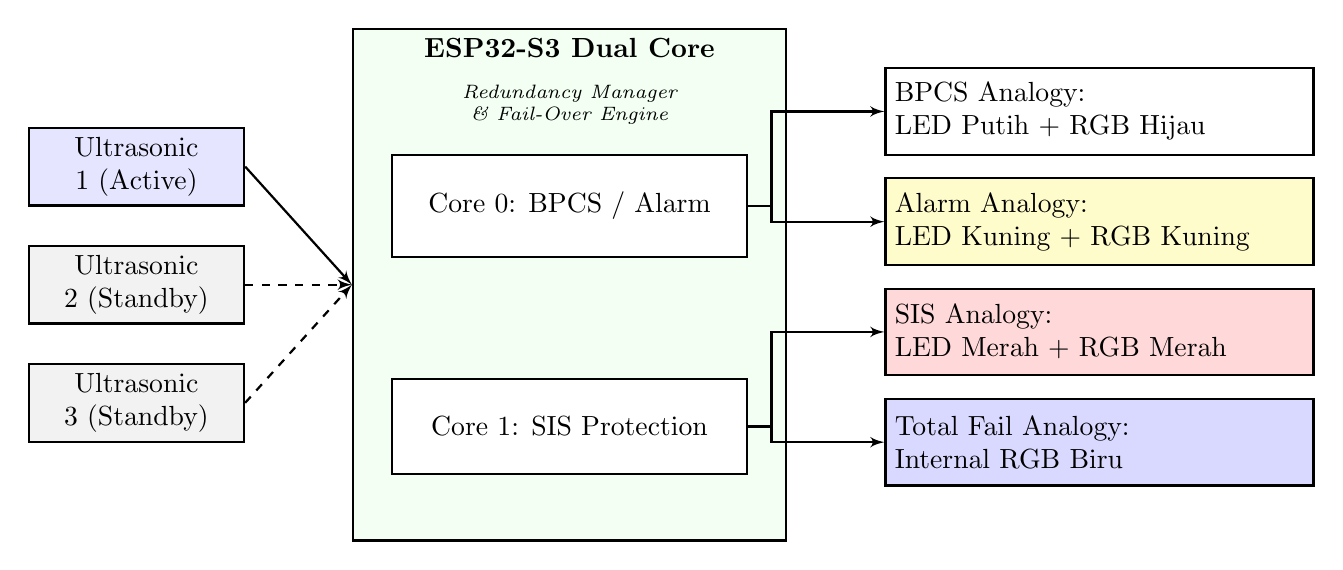
\begin{tikzpicture}[node distance=1.5cm, auto, >=latex', thick]
    % Sensors
    \node [draw, rectangle, fill=blue!10, text width=2.5cm, align=center] (s1) at (0,1.5) {Ultrasonic 1 (Active)};
    \node [draw, rectangle, fill=gray!10, text width=2.5cm, align=center] (s2) at (0,0) {Ultrasonic 2 (Standby)};
    \node [draw, rectangle, fill=gray!10, text width=2.5cm, align=center] (s3) at (0,-1.5) {Ultrasonic 3 (Standby)};
    
    % MCU Central Box
    \node [draw, rectangle, fill=green!5, minimum height=6.5cm, minimum width=5.5cm, align=center] (mcu) at (5.5,0) {};
    
    % MCU Labels (Internal)
    \node [anchor=north, font=\bfseries] at (mcu.north) {ESP32-S3 Dual Core};
    \node [anchor=north, font=\scriptsize\itshape, align=center] at ([yshift=-0.6cm]mcu.north) {Redundancy Manager \\ \& Fail-Over Engine};
    
    % MCU Sub-blocks
    \node [draw, rectangle, fill=white, minimum width=4.5cm, minimum height=1.3cm] (c0) at (5.5,1) {Core 0: BPCS / Alarm};
    \node [draw, rectangle, fill=white, minimum width=4.5cm, minimum height=1.2cm] (c1) at (5.5,-1.8) {Core 1: SIS Protection};

    % Output Analogy Blocks
    \node [draw, rectangle, fill=white, text width=5.2cm, anchor=west, minimum height=1.1cm] (out1) at (9.5,2.2) {BPCS Analogy: \\ LED Putih + RGB Hijau};
    \node [draw, rectangle, fill=yellow!20, text width=5.2cm, anchor=west, minimum height=1.1cm] (out2) at (9.5,0.8) {Alarm Analogy: \\ LED Kuning + RGB Kuning};
    \node [draw, rectangle, fill=red!15, text width=5.2cm, anchor=west, minimum height=1.1cm] (out3) at (9.5,-0.6) {SIS Analogy: \\ LED Merah + RGB Merah};
    \node [draw, rectangle, fill=blue!15, text width=5.2cm, anchor=west, minimum height=1.1cm] (out4) at (9.5,-2.0) {Total Fail Analogy: \\ Internal RGB Biru};

    % Connections: Sensors to MCU
    \draw [->] (s1.east) -- (mcu.west);
    \draw [dashed, ->] (s2.east) -- (mcu.west);
    \draw [dashed, ->] (s3.east) -- (mcu.west);
    
    % Connections: Cores to Outputs
    \draw [->] (c0.east) -- ++(0.3,0) |- (out1.west);
    \draw [->] (c0.east) -- ++(0.3,0) |- (out2.west);
    \draw [->] (c1.east) -- ++(0.3,0) |- (out3.west);
    \draw [->] (c1.east) -- ++(0.3,0) |- (out4.west);
\end{tikzpicture}
\caption{Arsitektur Redundansi dan Hirarki Analogi Aktuator Sistem Kendali Level Air Terintegrasi}
\end{figure}

\noindent \textbf{Penjelasan Diagram Blok Sistem:}

Diagram blok pada Gambar 1 merepresentasikan arsitektur sistem kendali level air terintegrasi dengan tingkat integritas tinggi. Komponen sistem dibagi menjadi empat tahap utama:

\begin{enumerate}
    \item \textbf{Input Stage (Sensor Redundansi):} Sistem menggunakan tiga sensor ultrasonik HC-SR04 yang dikonfigurasi dalam mode \textit{Cold Redundancy}. \textit{Ultrasonic 1} bertindak sebagai sensor aktif utama, sementara \textit{Ultrasonic 2} dan \textit{3} berada dalam status \textit{standby} tanpa catu daya aktif untuk menghemat profil energi. Jika sensor aktif mengalami kegagalan pembacaan, sistem secara otomatis melakukan \textit{fail-over} ke sensor berikutnya.
    
    \item \textbf{Processing Stage (ESP32-S3 Dual Core):} Inti pemrosesan menggunakan mikrokontroler ESP32-S3 yang diprogram menggunakan bahasa \textit{Rust}. Keunggulan \textit{dual-core} dimanfaatkan untuk isolasi fungsi:
    \begin{itemize}
        \item \textbf{Core 0 (BPCS/Alarm):} Menangani logika kendali rutin (\textit{Basic Process Control System}) dan ambang batas peringatan (\textit{Alarm}).
        \item \textbf{Core 1 (SIS):} Didedikasikan khusus untuk \textit{Safety Instrumented System} (SIS). Pemisahan inti ini menjamin bahwa jika \textit{Core 0} mengalami beban komputasi tinggi atau \textit{crash}, fungsi proteksi pada \textit{Core 1} tetap beroperasi secara independen.
    \end{itemize}
    
    \item \textbf{Control \& Safety Logic (Rust Engine):} Algoritma \textit{Redundancy Manager} dan \textit{Fail-Over Engine} berjalan di atas lapisan \textit{memory safety} Rust. Hal ini memastikan perpindahan antar sensor redundan tidak menyebabkan \textit{buffer overflow} atau korupsi data pada variabel kritis.
    
    \item \textbf{Output Stage (Analogi Aktuator):} Sebagai sistem simulasi, output direpresentasikan melalui hirarki indikator LED:
    \begin{itemize}
        \item \textbf{BPCS:} LED Putih dan RGB internal Hijau aktif saat level air normal (50-74\%).
        \item \textbf{Alarm:} LED Kuning aktif saat air mencapai zona waspada (75-89\%) disertai warna Kuning pada RGB internal.
        \item \textbf{SIS:} LED Merah aktif saat kondisi kritis ($\geq$ 90\%), memicu aksi proteksi darurat dan RGB internal Merah.
        \item \textbf{Total Fail:} RGB internal Biru menyala jika ketiga sensor redundan mengalami kerusakan fisik secara simultan.
    \end{itemize}
\end{enumerate}

\subsection*{4. Flowchart Algoritma}

\begin{figure}[H]
\centering
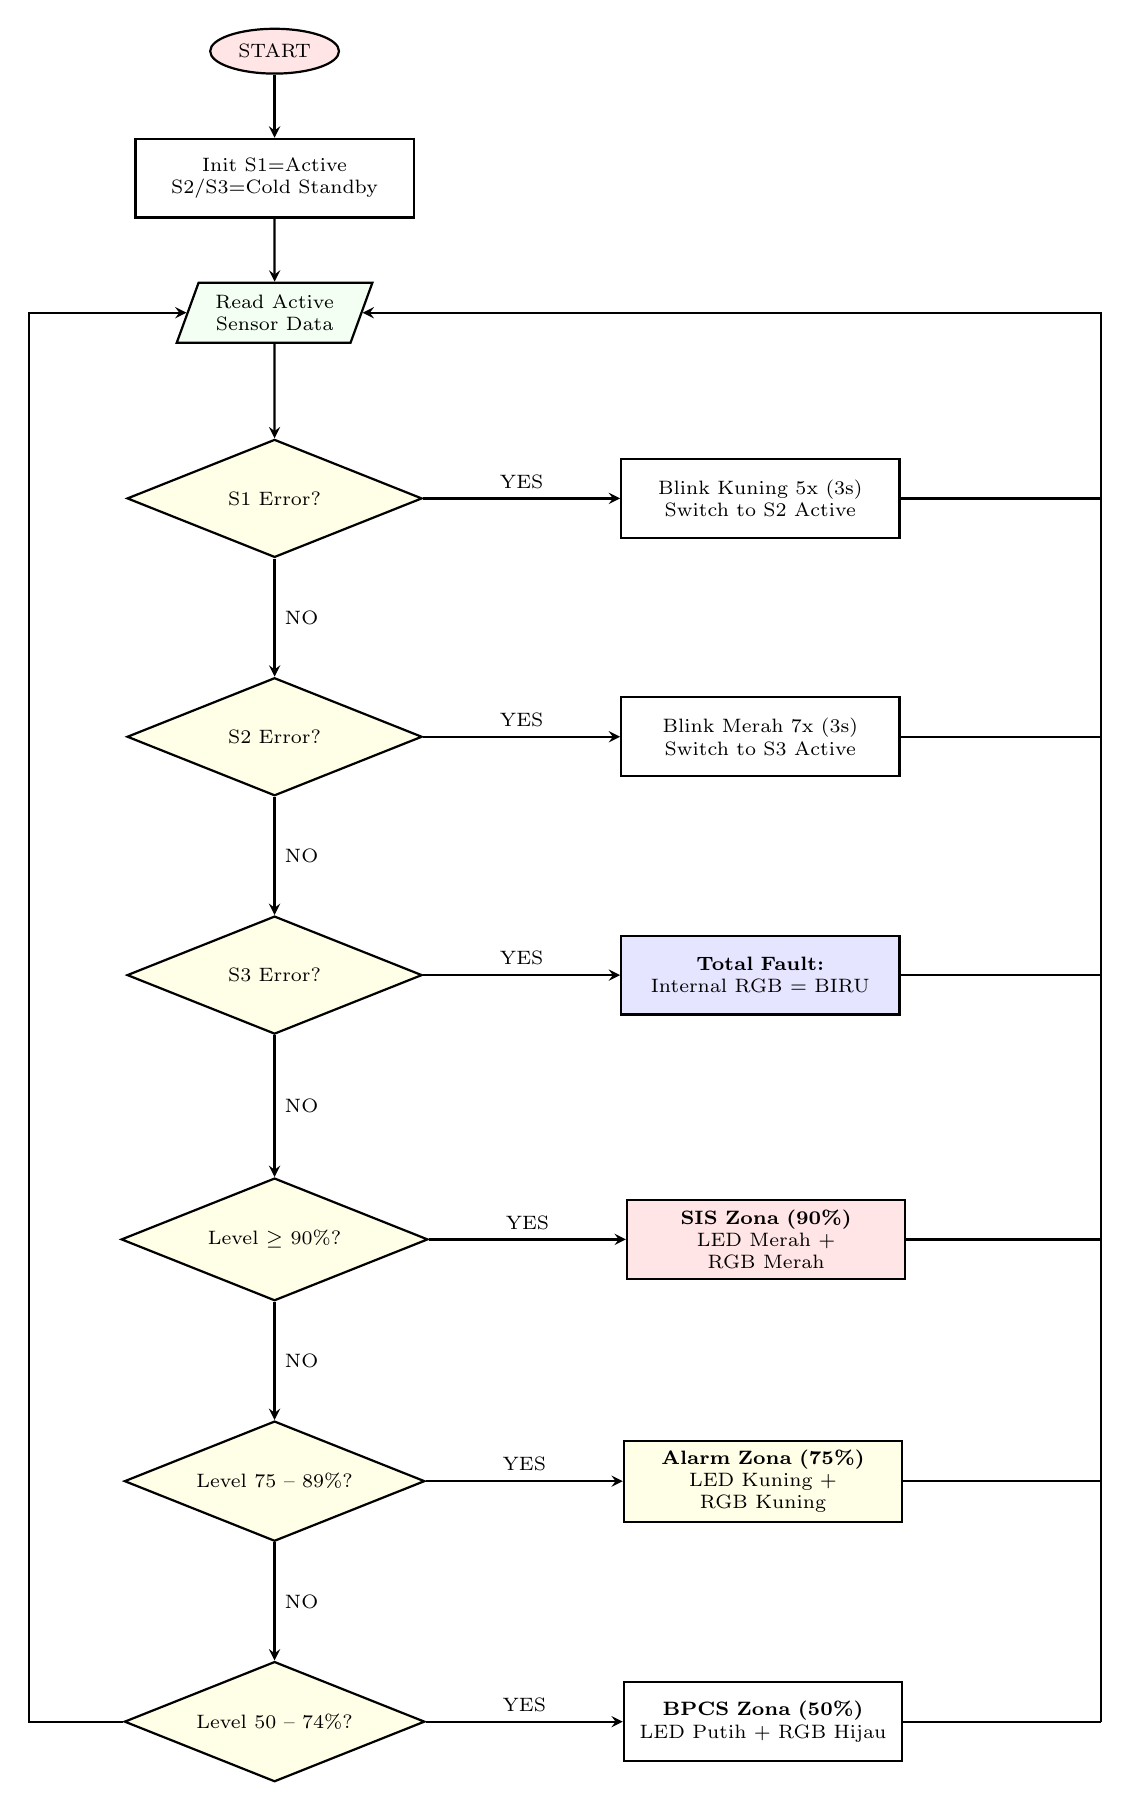
\begin{tikzpicture}[node distance=1.8cm, font=\scriptsize, >=stealth, thick]
    % Styles
    \tikzstyle{start} = [draw, ellipse, fill=red!10, minimum width=1.5cm]
    \tikzstyle{proc} = [draw, rectangle, fill=white, minimum width=3.2cm, text width=3.3cm, align=center, minimum height=1cm]
    \tikzstyle{decision} = [draw, diamond, aspect=2.5, fill=yellow!10, minimum width=3cm, text width=2.5cm, align=center]
    \tikzstyle{io} = [draw, trapezium, trapezium left angle=70, trapezium right angle=110, fill=green!5, minimum width=2.5cm, align=center]

    % Nodes
    \node (start) [start] {START};
    \node (init) [proc, below=0.8cm of start] {Init S1=Active \\ S2/S3=Cold Standby};
    \node (read) [io, below=0.8cm of init] {Read Active \\ Sensor Data};
    
    % S1 Logic
    \node (fail1) [decision, below=1.2cm of read] {S1 Error?};
    \node (blink1) [proc, right=2.5cm of fail1] {Blink Kuning 5x (3s) \\ Switch to S2 Active};
    
    % S2 Logic
    \node (fail2) [decision, below=1.5cm of fail1] {S2 Error?};
    \node (blink2) [proc, right=2.5cm of fail2] {Blink Merah 7x (3s) \\ Switch to S3 Active};
    
    % S3 Logic
    \node (fail3) [decision, below=1.5cm of fail2] {S3 Error?};
    \node (allfail) [proc, right=2.5cm of fail3, fill=blue!10] {\textbf{Total Fault:} \\ Internal RGB = BIRU};

    % Sequential Level Check
    \node (level1) [decision, below=1.8cm of fail3] {Level $\geq$ 90\%?};
    \node (sis) [proc, right=2.5cm of level1, fill=red!10] {\textbf{SIS Zona (90\%)} \\ LED Merah + RGB Merah};
    
    \node (level2) [decision, below=1.5cm of level1] {Level 75 -- 89\%?};
    \node (alarm) [proc, right=2.5cm of level2, fill=yellow!10] {\textbf{Alarm Zona (75\%)} \\ LED Kuning + RGB Kuning};
    
    \node (level3) [decision, below=1.5cm of level2] {Level 50 -- 74\%?};
    \node (bpcs) [proc, right=2.5cm of level3, fill=white] {\textbf{BPCS Zona (50\%)} \\ LED Putih + RGB Hijau};

    % BUS coordinate for right-side return line (further to the right to avoid boxes)
    \coordinate (bus) at (10.5,0); 

    % Paths: Decision Flow
    \draw [->] (start) -- (init);
    \draw [->] (init) -- (read);
    \draw [->] (read) -- (fail1);
    
    \draw [->] (fail1) -- node[anchor=south] {YES} (blink1);
    \draw [->] (fail1) -- node[anchor=west] {NO} (fail2);
    
    \draw [->] (fail2) -- node[anchor=south] {YES} (blink2);
    \draw [->] (fail2) -- node[anchor=west] {NO} (fail3);
    
    \draw [->] (fail3) -- node[anchor=south] {YES} (allfail);
    \draw [->] (fail3) -- node[anchor=west] {NO} (level1);
    
    \draw [->] (level1) -- node[anchor=south] {YES} (sis);
    \draw [->] (level1) -- node[anchor=west] {NO} (level2);
    
    \draw [->] (level2) -- node[anchor=south] {YES} (alarm);
    \draw [->] (level2) -- node[anchor=west] {NO} (level3);

    \draw [->] (level3) -- node[anchor=south] {YES} (bpcs);
    
    % Return from NO level3 (Looping back to read)
    \draw [->] (level3.west) -- ++(-1.2,0) |- (read.west); 
    
    % Merged Return Bus on the Right
    \draw [-] (blink1.east) -- (blink1.east -| bus);
    \draw [-] (blink2.east) -- (blink2.east -| bus);
    \draw [-] (allfail.east) -- (allfail.east -| bus);
    \draw [-] (sis.east) -- (sis.east -| bus);
    \draw [-] (alarm.east) -- (alarm.east -| bus);
    \draw [-] (bpcs.east) -- (bpcs.east -| bus);
    
    % The Merged Bus vertical line returning to Read
    \draw [->] (bpcs.east -| bus) -- (bus |- read.east) -- (read.east);

\end{tikzpicture}
\caption{Flowchart Logika Sequential Manajemen Redundansi dan Hirarki Proteksi}
\end{figure}

\noindent \textbf{Penjelasan Flowchart Algoritma:}

Flowchart pada Gambar 2 menjelaskan alur logika sistem dari inisialisasi hingga pengambilan keputusan keamanan secara bertingkat. Proses algoritma dirancang untuk menjamin \textit{high availability} melalui mekanisme berikut:

\begin{enumerate}
    \item \textbf{Inisialisasi dan Inisiasi Cold Redundancy:} Sistem dimulai dengan menetapkan Sensor 1 (S1) sebagai unit aktif. Untuk efisiensi energi (\textit{Cold Redundancy}), Sensor 2 (S2) dan Sensor 3 (S3) tetap berada dalam kondisi mati (\textit{OFF}) hingga dibutuhkan.
    
    \item \textbf{Mekanisme Deteksi Kegagalan (Fail-Over Logic):} Sistem secara kontinu memeriksa validitas data dari sensor yang aktif. Jika terjadi galat (\textit{Error}):
    \begin{itemize}
        \item \textbf{Transisi S1 ke S2:} LED kuning berkedip (\textit{blink}) 5 kali dalam durasi 3 detik sebagai peringatan kegagalan fisik pertama, kemudian S2 diaktifkan.
        \item \textbf{Transisi S2 ke S3:} Jika S2 juga gagal, LED merah berkedip 7 kali dalam 3 detik, dan sistem berpindah ke sensor redundan terakhir (S3).
        \item \textbf{Total Fault:} Jika S3 gagal, sistem memasuki mode darurat kritis di mana RGB internal ESP32-S3 menyala Biru secara statis untuk menandakan hilangnya seluruh data sensor.
    \end{itemize}

    \item \textbf{Hirarki Pengendalian Sequential (BPCS, Alarm, SIS):} Setelah data sensor divalidasi, sistem melakukan pengecekan level air secara berurutan:
    \begin{itemize}
        \item \textbf{SIS ($\geq$ 90\%):} Air mencapai ambang batas kritis. Sistem mengaktifkan LED Merah dan RGB internal Merah.
        \item \textbf{Alarm (75-89\%):} Sistem memberikan peringatan melalui LED Kuning dan RGB internal Kuning.
        \item \textbf{BPCS (50-74\%):} Sistem berada dalam kendali rutin ditandai dengan LED Putih dan RGB internal Hijau.
        \item \textbf{Normal (< 50\%):} Level air aman, hanya RGB internal Hijau yang aktif sebagai indikator daya.
    \end{itemize}
\end{enumerate}

\newpage
\section*{C. Simulasi dan Hasil}

\subsection*{1. Alat dan Bahan}
Sistem ini diimplementasikan menggunakan komponen berikut:
\begin{itemize}
    \item \textbf{Hardware:} ESP32-S3 (Dual Core LX7), 3 Sensor Ultrasonik HC-SR04, LED (Putih, Kuning, Merah), Resistor 220$\Omega$.
    \item \textbf{Software:} Visual Studio Code (IDE), Rust Toolchain (\textit{esp-rs}), Wokwi.
\end{itemize}

\begin{small}
\begin{table}[H]
\centering
\caption{Spesifikasi Teknis Mikrokontroler ESP32-S3}
\begin{tabular}{|l|l|}
\hline
\textbf{Fitur} & \textbf{Deskripsi Spesifikasi} \\ \hline
Prosesor & Dual-core Xtensa® 32-bit LX7 CPU \\ \hline
Kecepatan Clock & Hingga 240 MHz \\ \hline
Memori & 512 KB SRAM, 384 KB ROM, 16 KB RTC SRAM \\ \hline
Konektivitas & Wi-Fi 2.4 GHz \& Bluetooth 5 (LE) \\ \hline
Periferal & 45 GPIO, ADC, PWM, I2C, SPI, UART, RMT \\ \hline
\end{tabular}
\end{table}

\begin{table}[H]
\centering
\caption{Spesifikasi Teknis Sensor Ultrasonik HC-SR04}
\begin{tabular}{|l|l|}
\hline
\textbf{Parameter} & \textbf{Nilai Spesifikasi} \\ \hline
Tegangan Operasional & DC 5V \\ \hline
Arus Operasional & 15 mA \\ \hline
Frekuensi Kerja & 40 kHz \\ \hline
Jarak Pengukuran & 2 cm -- 400 cm \\ \hline
Sinyal Input Trigger & 10$\mu$s Pulsa TTL \\ \hline
\end{tabular}
\end{table}
\end{small}

\subsection*{2. Dokumentasi Pengujian Sensor 1 (Utama)}
\begin{figure}[H]
    \centering
    \begin{subfigure}[b]{0.45\textwidth}
        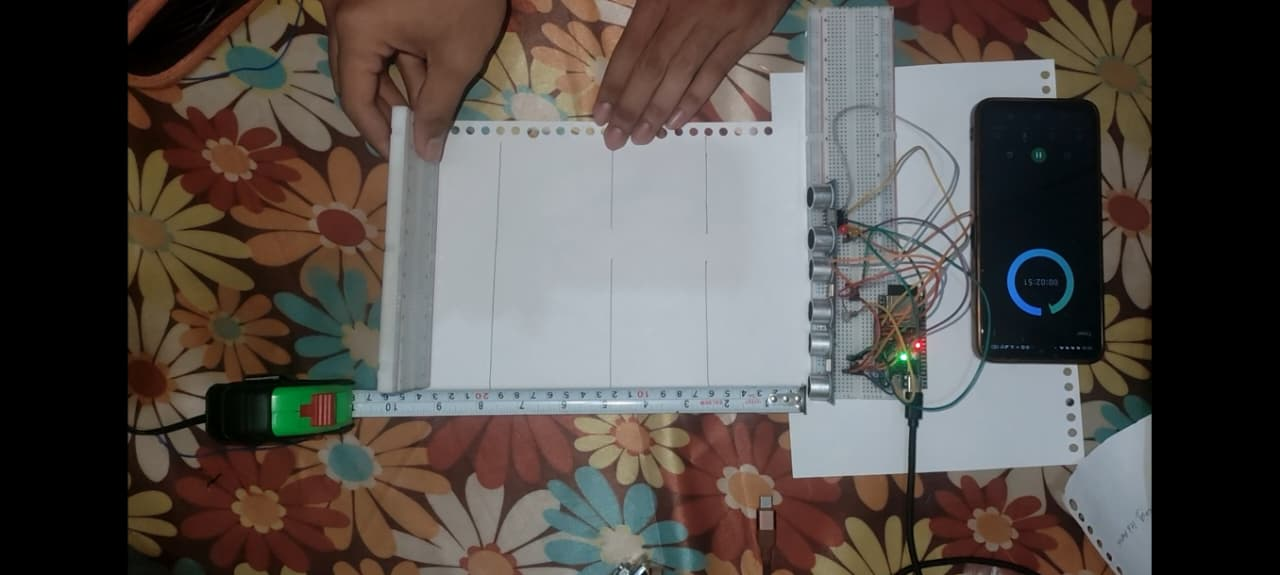
\includegraphics[width=\textwidth]{Sensor1/Normal_S1.jpeg}
        \caption{Normal (< 50\%)}
    \end{subfigure}
    \hfill
    \begin{subfigure}[b]{0.45\textwidth}
        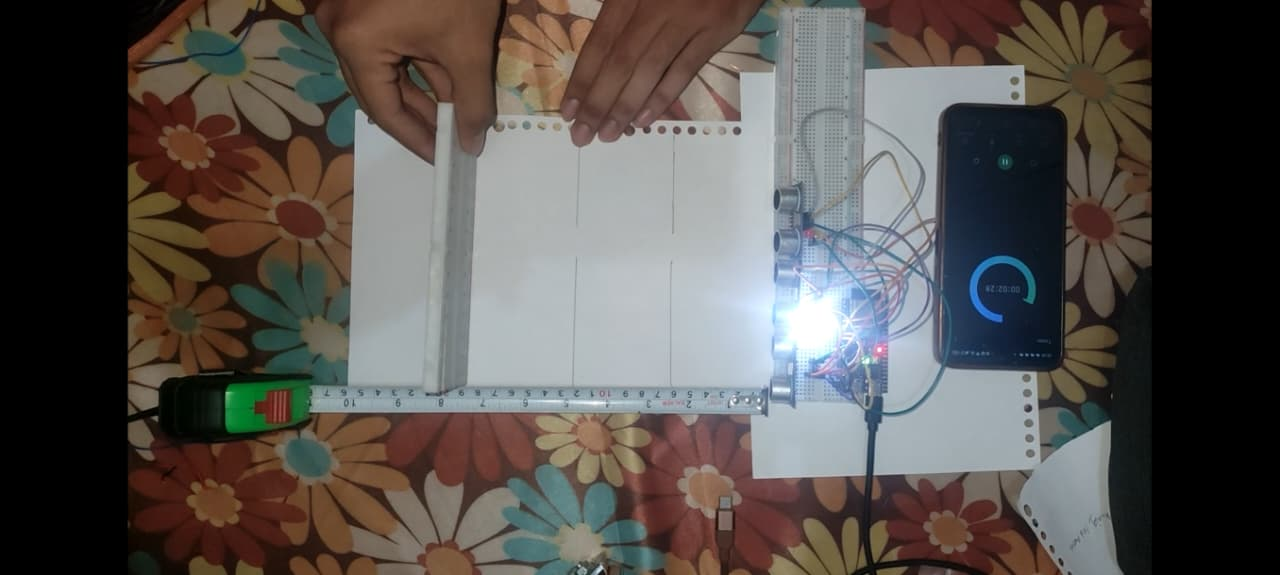
\includegraphics[width=\textwidth]{Sensor1/BPCS_S1.jpeg}
        \caption{BPCS (50-74\%)}
    \end{subfigure}
    \\[10pt]
    \begin{subfigure}[b]{0.45\textwidth}
        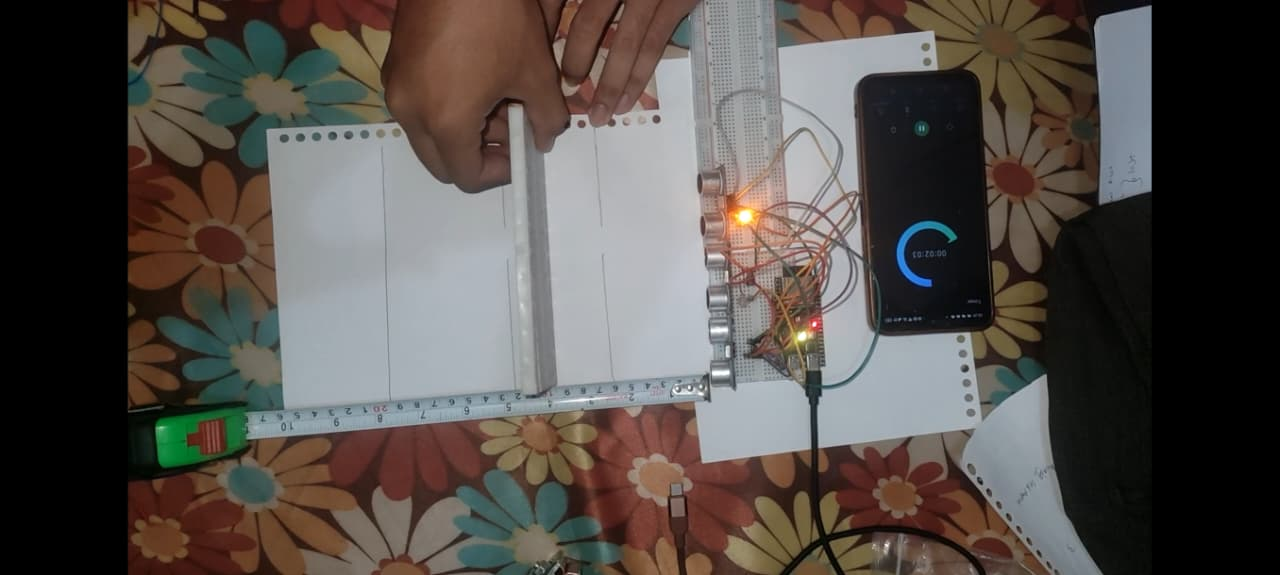
\includegraphics[width=\textwidth]{Sensor1/ALARM_S1.jpeg}
        \caption{ALARM (75-89\%)}
    \end{subfigure}
    \hfill
    \begin{subfigure}[b]{0.45\textwidth}
        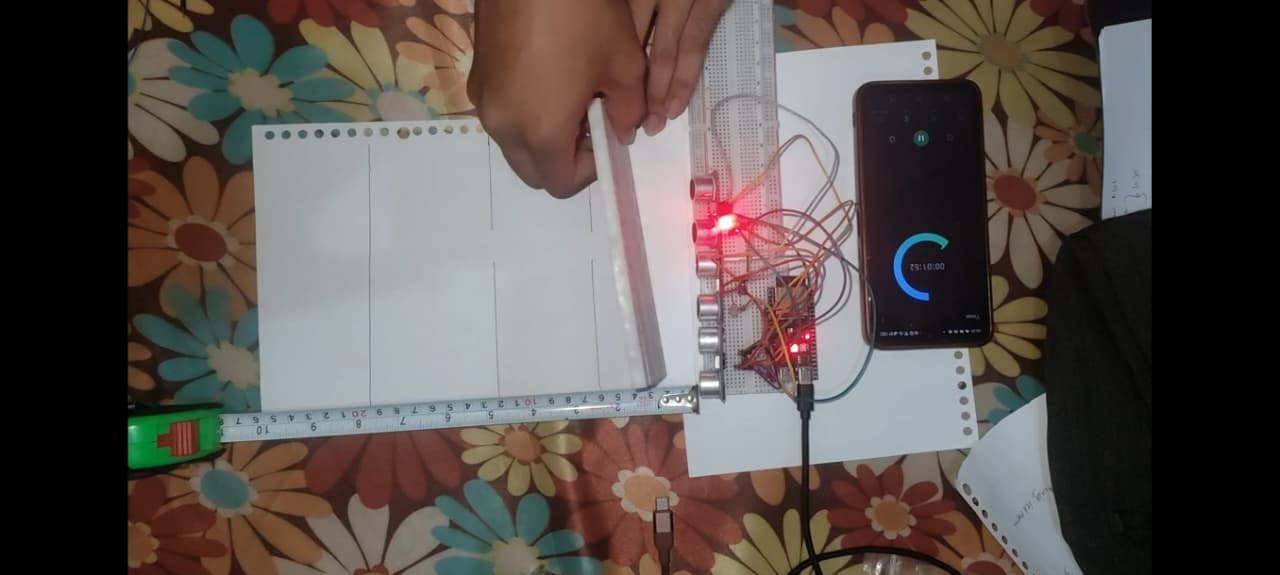
\includegraphics[width=\textwidth]{Sensor1/SIS_S1.jpeg}
        \caption{SIS ($\geq$ 90\%)}
    \end{subfigure}
    \\[10pt]
    \begin{subfigure}[b]{0.45\textwidth}
        \centering
        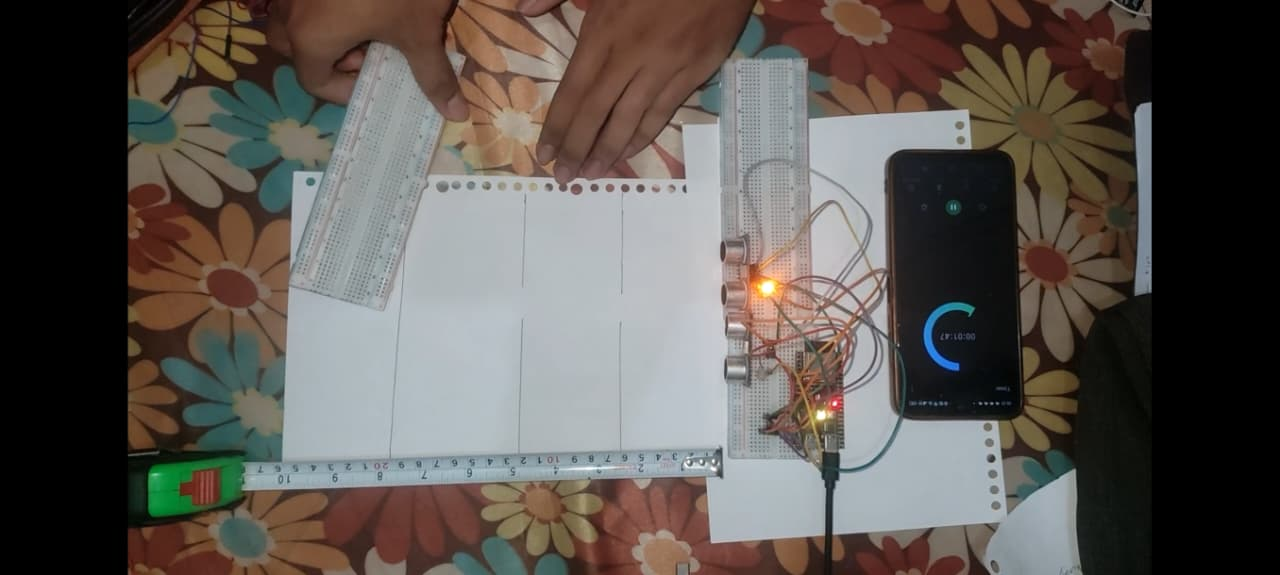
\includegraphics[width=\textwidth]{Sensor1/SwitchS1-S2.jpeg}
        \caption{S1 Error $\rightarrow$ Switch S2}
    \end{subfigure}
    \caption{Skenario Simulasi Menggunakan Sensor 1}
\end{figure}

\subsection*{3. Dokumentasi Pengujian Sensor 2 (Redundansi 1)}
\begin{figure}[H]
    \centering
    \begin{subfigure}[b]{0.45\textwidth}
        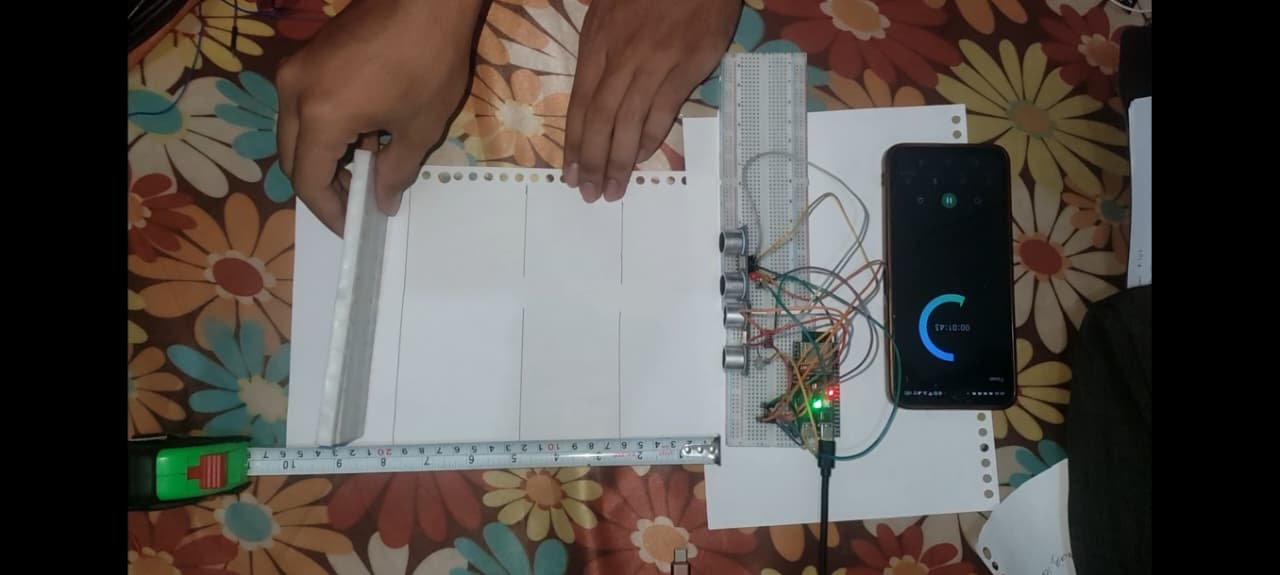
\includegraphics[width=\textwidth]{Sensor2/Normal_S2.jpeg}
        \caption{Normal (< 50\%)}
    \end{subfigure}
    \hfill
    \begin{subfigure}[b]{0.45\textwidth}
        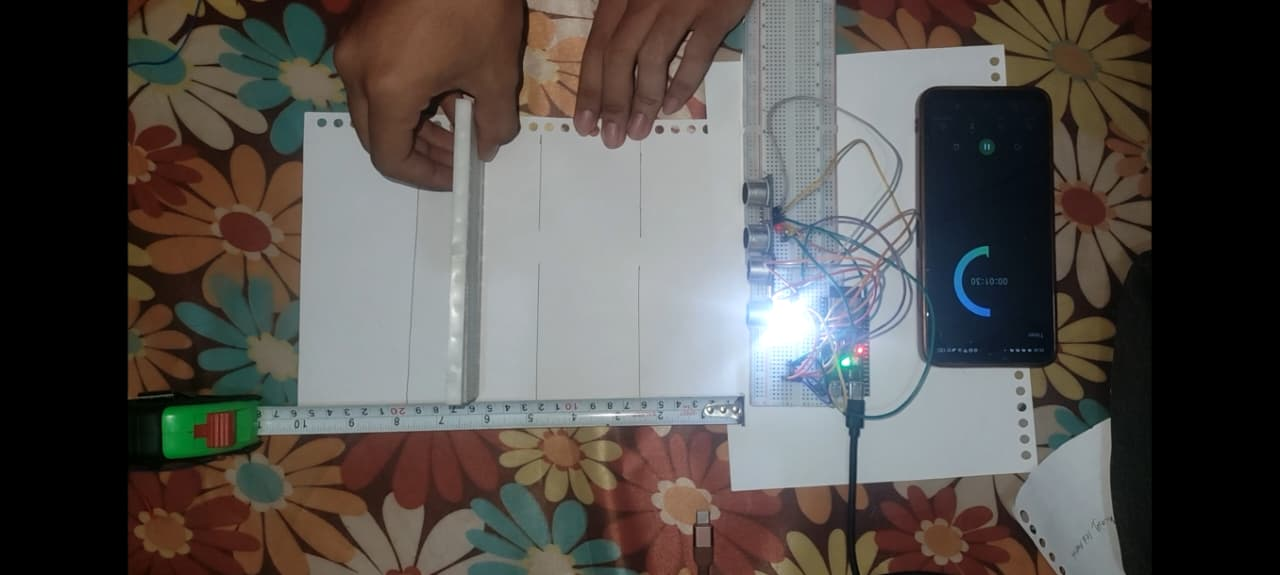
\includegraphics[width=\textwidth]{Sensor2/BPCS_S2.jpeg}
        \caption{BPCS (50-74\%)}
    \end{subfigure}
    \\[10pt]
    \begin{subfigure}[b]{0.45\textwidth}
        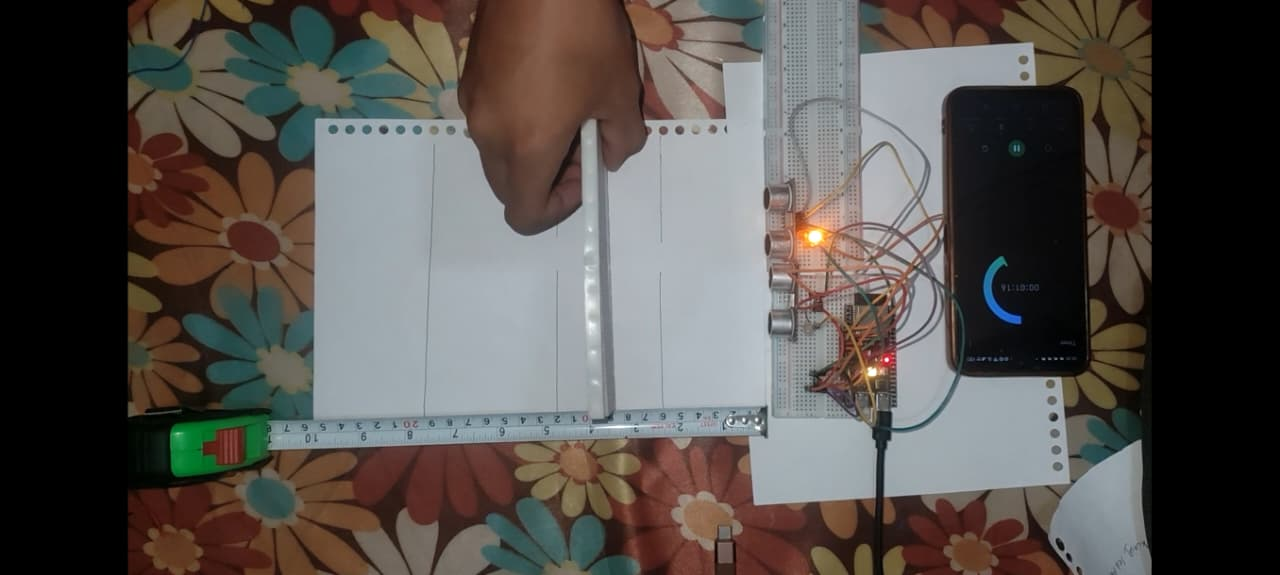
\includegraphics[width=\textwidth]{Sensor2/ALARM_S2.jpeg}
        \caption{ALARM (75-89\%)}
    \end{subfigure}
    \hfill
    \begin{subfigure}[b]{0.45\textwidth}
        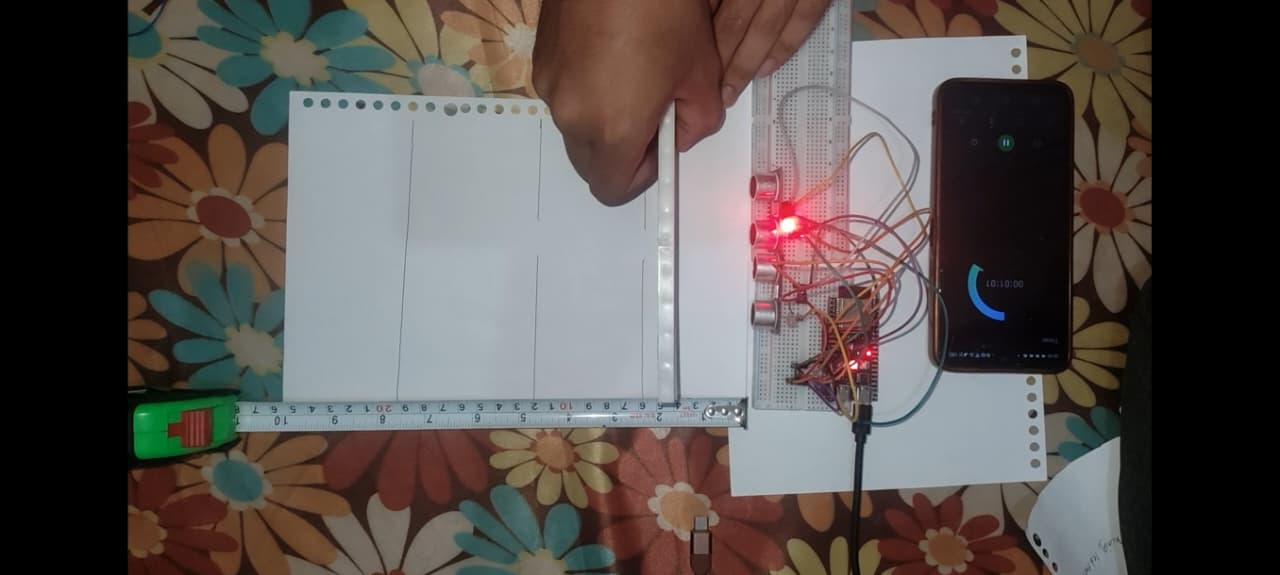
\includegraphics[width=\textwidth]{Sensor2/SIS_S2.jpeg}
        \caption{SIS ($\geq$ 90\%)}
    \end{subfigure}
    \\[10pt]
    \begin{subfigure}[b]{0.45\textwidth}
        \centering
        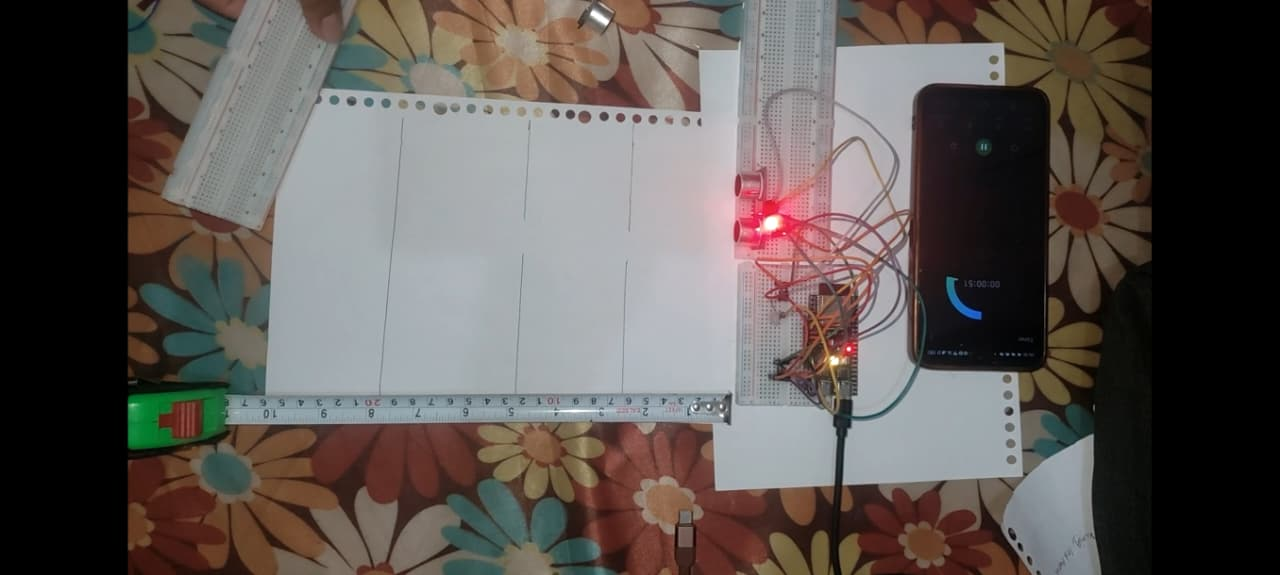
\includegraphics[width=\textwidth]{Sensor2/SwitchS2-S3.jpeg}
        \caption{S2 Error $\rightarrow$ Switch S3}
    \end{subfigure}
    \caption{Skenario Simulasi Menggunakan Sensor 2}
\end{figure}

\subsection*{4. Dokumentasi Pengujian Sensor 3 dan Kegagalan Total}
\begin{figure}[H]
    \centering
    \begin{subfigure}[b]{0.45\textwidth}
        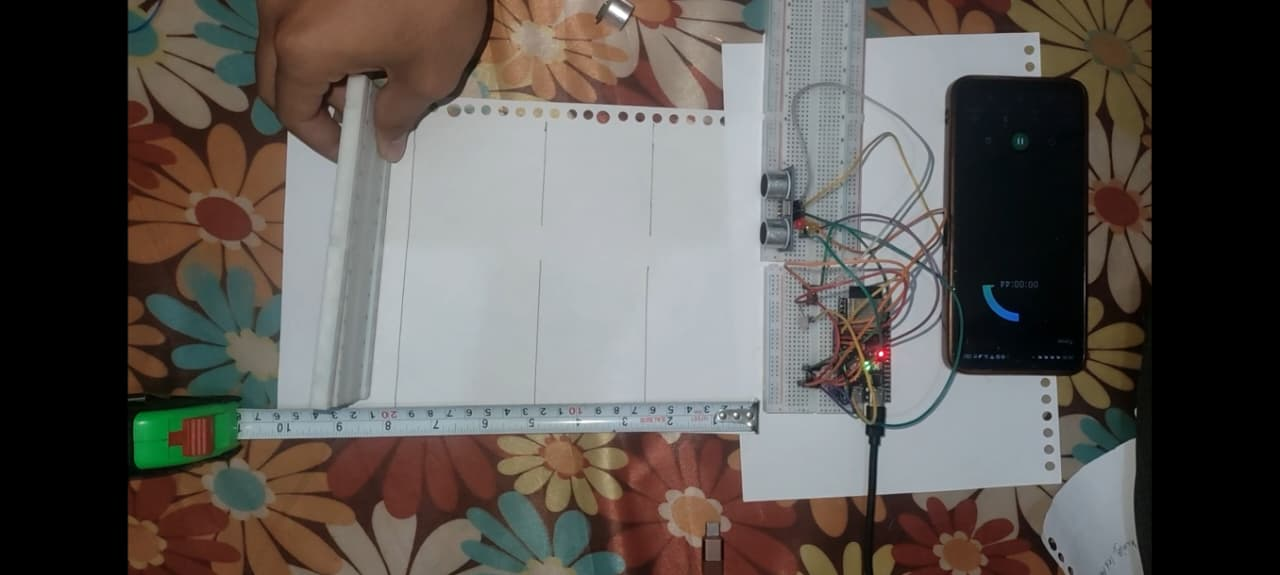
\includegraphics[width=\textwidth]{Sensor3/Normal_S3.jpeg}
        \caption{Normal (< 50\%)}
    \end{subfigure}
    \hfill
    \begin{subfigure}[b]{0.45\textwidth}
        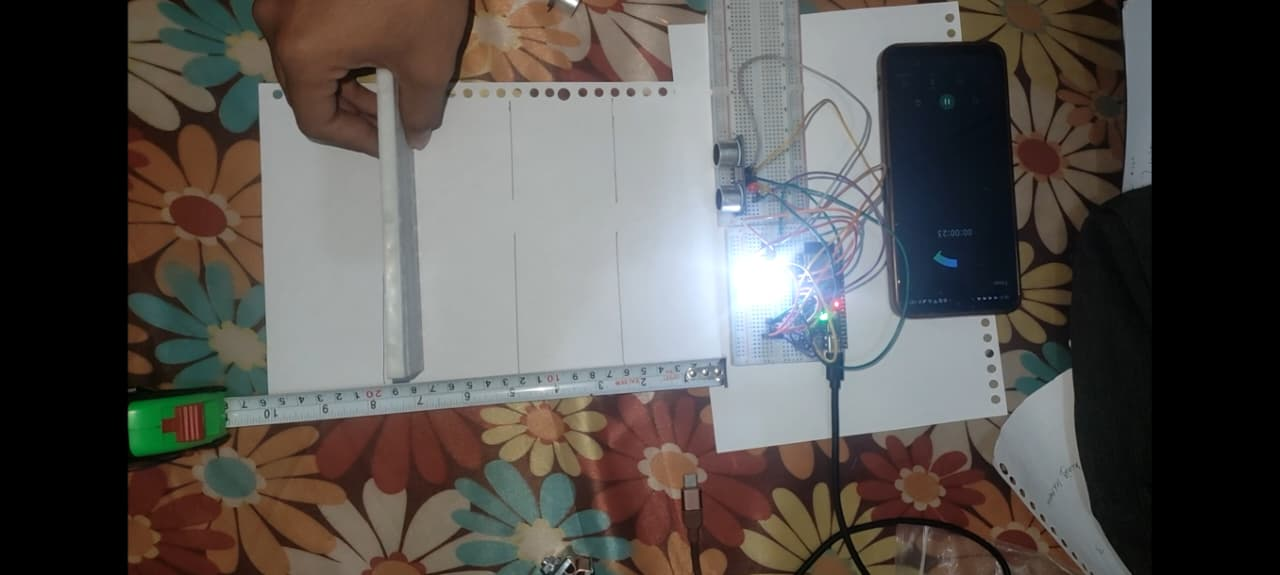
\includegraphics[width=\textwidth]{Sensor3/BPCS_S3.jpeg}
        \caption{BPCS (50-74\%)}
    \end{subfigure}
    \\[10pt]
    \begin{subfigure}[b]{0.45\textwidth}
        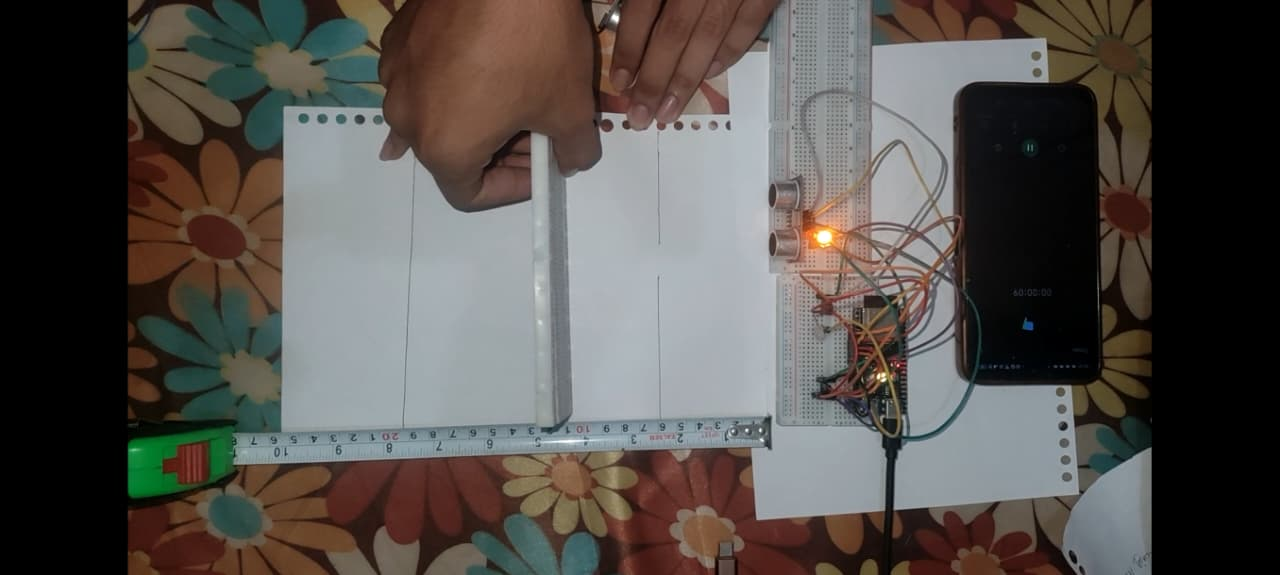
\includegraphics[width=\textwidth]{Sensor3/ALARM_S3.jpeg}
        \caption{ALARM (75-89\%)}
    \end{subfigure}
    \hfill
    \begin{subfigure}[b]{0.45\textwidth}
        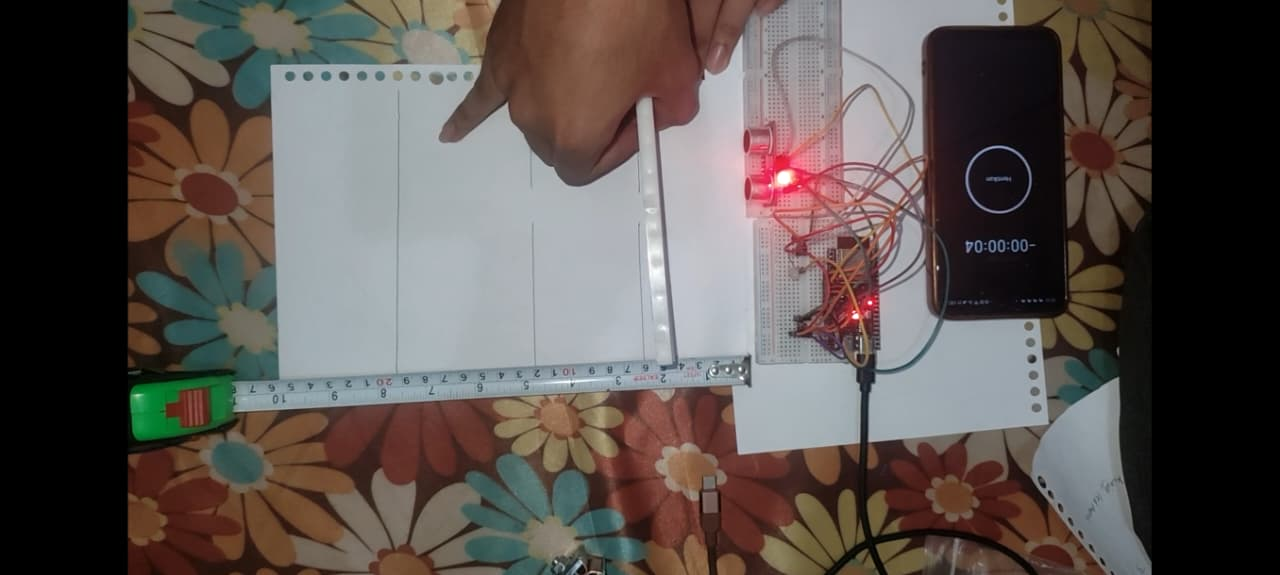
\includegraphics[width=\textwidth]{Sensor3/SIS_S3.jpeg}
        \caption{SIS ($\geq$ 90\%)}
    \end{subfigure}
    \\[10pt]
    \begin{subfigure}[b]{0.45\textwidth}
        \centering
        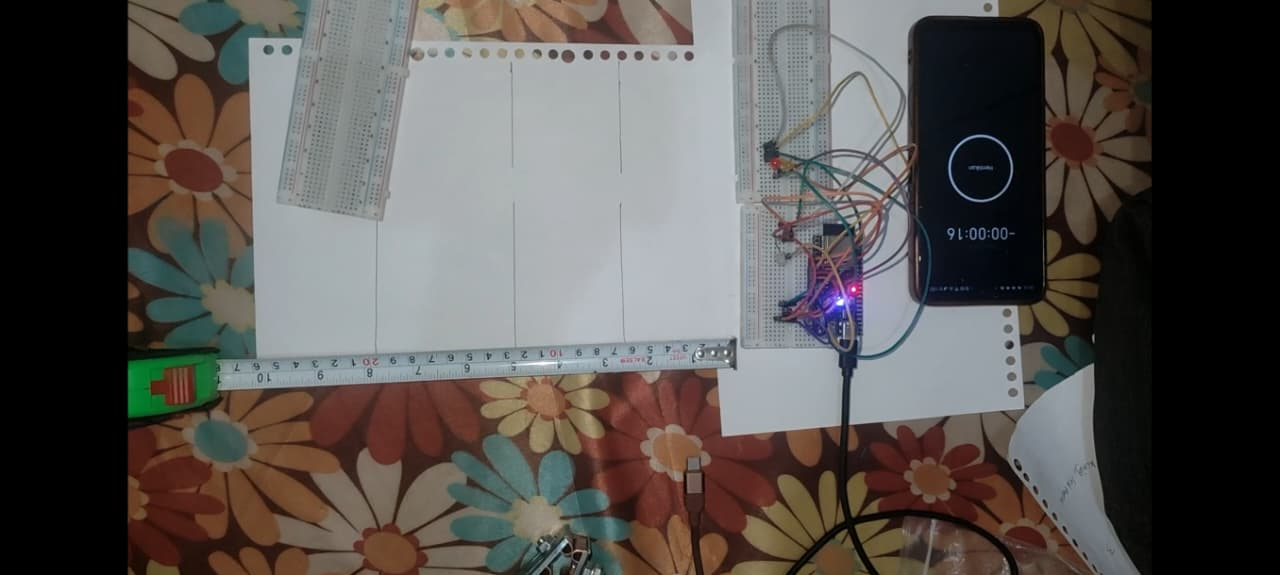
\includegraphics[width=\textwidth]{Sensor3/TanpaSensor.jpeg}
        \caption{Kegagalan Total (Internal Biru)}
    \end{subfigure}
    \caption{Skenario Simulasi Menggunakan Sensor 3 dan Kondisi Akhir}
\end{figure}

\newpage
\section*{D. Keunggulan Metode}
1. \textbf{Redundansi Cerdas:} Strategi \textit{Cold Redundancy} meminimalkan konsumsi energi sekaligus menjaga ketersediaan sistem instrumentasi tanpa interferensi antar sensor. \\
2. \textbf{Diagnostik Visual Intuitif:} Pola \textit{blink} yang berbeda (5x dan 7x) memudahkan operator simulasi mengidentifikasi kegagalan fisik sensor redundan tanpa alat diagnostik tambahan. \\
3. \textbf{Keamanan Memori dan Integritas Tinggi:} Penggunaan Rust menjamin tidak adanya kebocoran memori (\textit{memory leaks}) dan \textit{undefined behavior} saat terjadi transisi antar sensor redundan.

\section*{E. Kesimpulan}
Sistem Redundant Integrated Basic Process Control System (BPCS) and Safety Instrumented System (SIS) Architecture membuktikan bahwa strategi redundansi sensor industri dapat diimplementasikan secara efisien pada ESP32-S3 menggunakan bahasa Rust. Penggunaan LED sebagai analogi aktuator mempermudah validasi hirarki perlindungan sistem (BPCS, Alarm, SIS) dan logika \textit{fail-over} dalam lingkungan simulasi yang aman, andal, dan memiliki integritas tinggi.

\end{document}
--- END OF FILE ---